\section{Thursday, April 13th: Collaboration and Social Computing}
\subsection{Post Midterm 2 Feedback Form}
Please fill out the form pinned on EdStem if you have anything to share!

\subsection{Remote Communication}
\subsubsection{Zoom}
We all are familiar with online meetings over Zoom.


\subsubsection{Collaboration Apps}
\begin{itemize}
    \item A lot of big companies fell behind because they did not allow for collaboration (ex. Microsoft Word falling behind Google Docs)
    \begin{itemize}
        \item The companies have tried to make up for it (Word now allows collaboration) but it hasn't been enough -- the software wasn't \textbf{designed} for collaboration \textit{from the start}.
        \item This was an easy way to make a lot of money in the early days of (EE)CS -- make a new product which is just an existing product but with collaboration
    \end{itemize}
\end{itemize}

\subsubsection{Calendars}
\begin{shaded}
Who here uses a Google Calendar (or some equivalent) to manage your schedule?
\end{shaded}
As expected, almost everyone in the room raised their hand.

The ability to anonymize what you are doing (and thus not have to worry about people scheduling events they think are `more important' over your existing events) was a key factor in its popularity.


\subsection{Challenges to social software}
\subsubsection{Success crisis}
\begin{shaded}
    Whether your software scales will only become apparent once you are successful, and then it’s often too late to change the architecture (see Friendster)
\end{shaded}
This is somewhat reminiscent of ``Design security in from the start'' from CS 161.

\subsection{Single Display Groupware}
\subsubsection{Roomware}
Example: AT\&T Network Center Control Room -- has everyone in the same room at the same time, even if they have different responsibilities. This helps develop a shared sense of purpose for the end-goal and allows people to be up to the date wth the overall project status.

\subsection{Graph Theory}
\begin{itemize}
    \item  \# of edges in a fully connected graph: $n*(n-1)/2 \quad\sim n^2$
    \item \# of edges in a tree: $n-1$
\end{itemize}

\begin{shaded}
    \textbf{Coasean Floor}: The point below which the transaction costs of a particular type of activity are too high for a standard institution to pursue.
    $\hfill\text{- Clay Shirky}$
\end{shaded}

\subsection{Power Law Distributions}
\begin{center}
    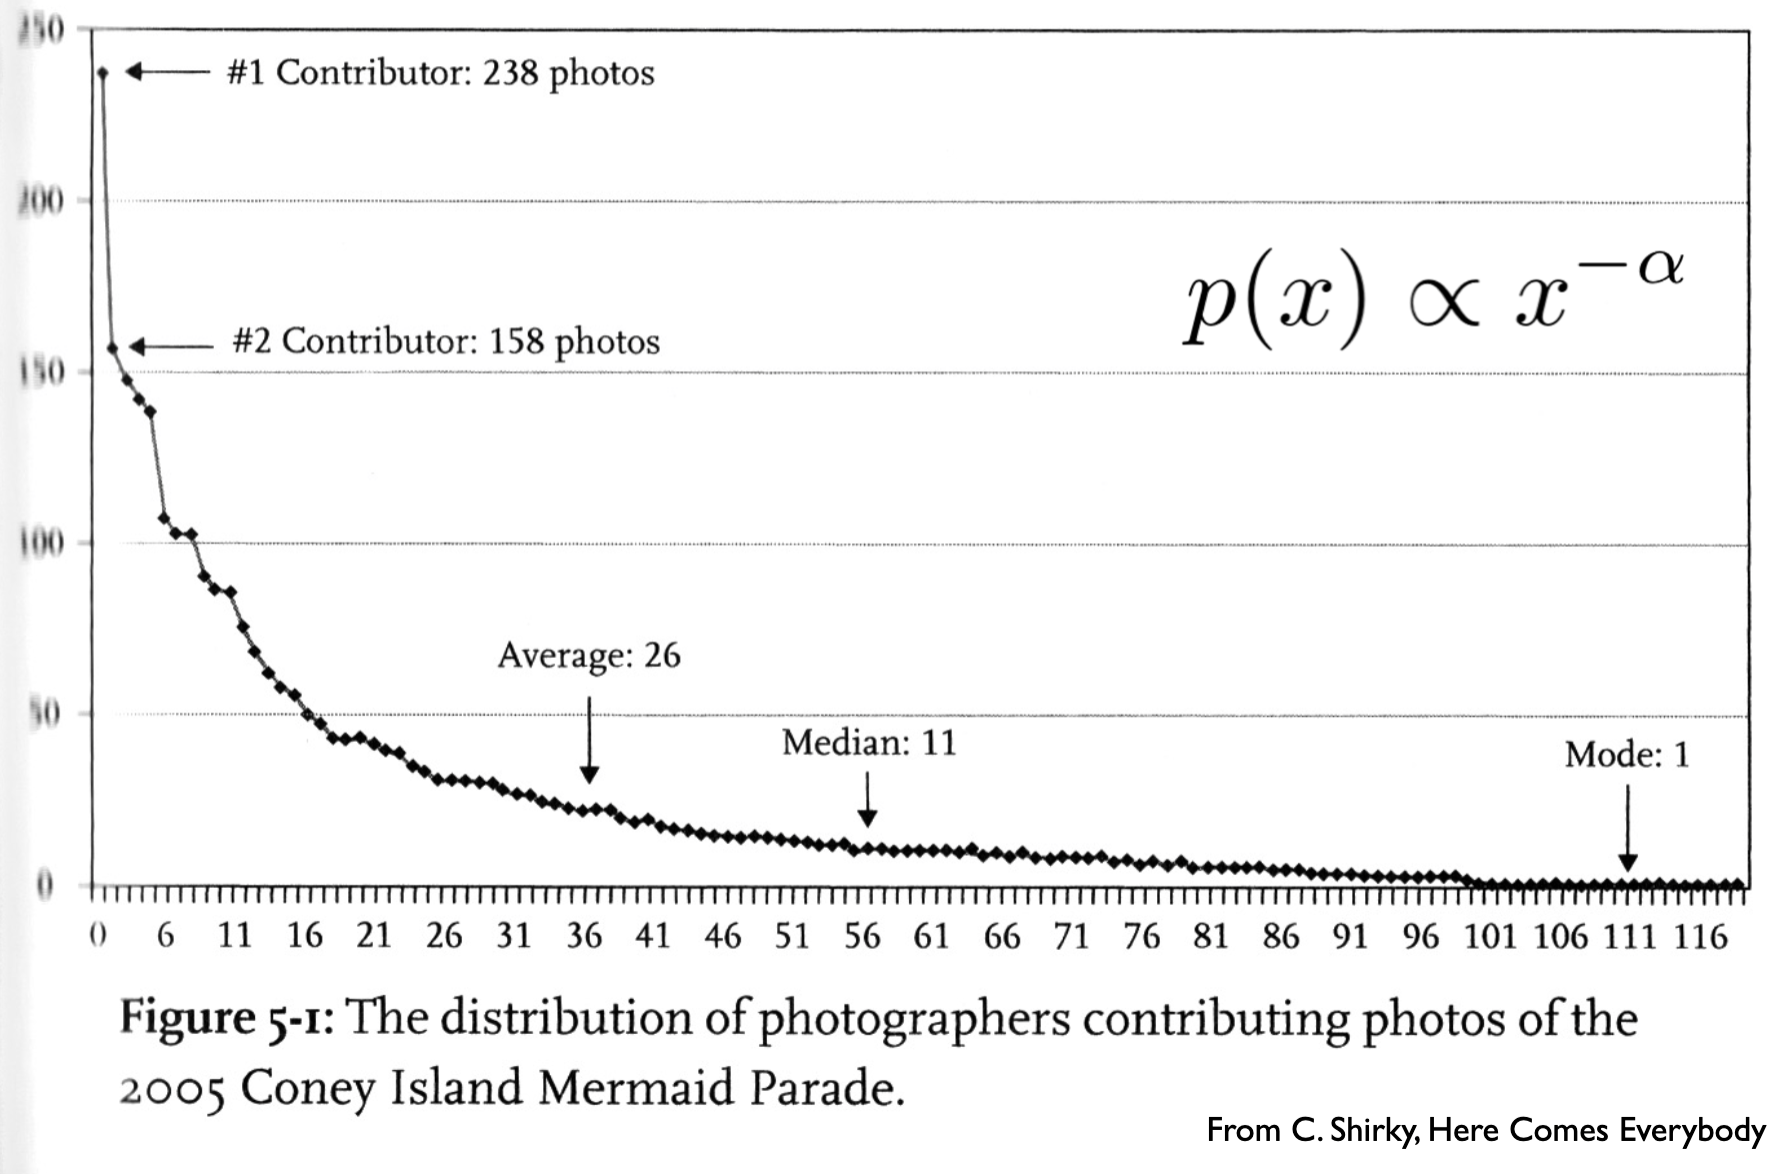
\includegraphics[scale=0.5]{lectures/wk12/img/pl_distro.png}
\end{center}
\[
p(x)\propto x^{-\alpha}
\]

\subsection{Time/Space Matrix}
\begin{tabular}{ |s|l|l| }
\hline
 & Same time (synchronous) & Different time (asynchronous) \\
\hline
{Same place \newline(co-located)} & Face-to-face interactions & Continuous Task \\
\hline
{Different place \newline(remote)} & Remote interactions & Communication + Coordination \\
\hline
\end{tabular}

\subsubsection{There goes the neighborhood:}
\begin{shaded}
Early adopters are often a self-selected, homogenous group; therefore utility in early stages is not indicative of the ``steady state'' once successful.
\end{shaded}
When new people use your app, they may say `there goes the neighborhood' to express how they feels new users will be detrimental to the app, due to them using the app in unintended ways.
